% \documentclass[table]{beamer}
\documentclass[table,handout]{beamer}
\setbeameroption{show notes}
% \setbeameroption{hide notes}
% \setbeameroption{show only notes}
\usepackage{varwidth}

\newif\ifhide
\newif\ifpost
\newif\ifhideclicker

% \hidetrue
% \hideclickertrue
% \posttrue

\newcommand{\whiteout}[1]{\textcolor{white}{#1}}
% \newcommand{\whiteoutbox}[1]{\fcolorbox{white}{white}{\parbox{\dimexpr \linewidth-2\fboxsep-2\fboxrule}{\whiteout{#1}}}}
% \newcommand{\notebox}[1]{\fcolorbox{blue}{white}{\parbox{\dimexpr \linewidth-2\fboxsep-2\fboxrule}{#1}}}
\newcommand{\whiteoutbox}[1]{\fcolorbox{white}{white}{\parbox{\linewidth}{\whiteout{#1}}}}
\newcommand{\notebox}[1]{\fcolorbox{blue}{white}{\parbox{\linewidth}{#1}}}
\newcommand{\blankbox}[1]{\phantom{\varwidth{\linewidth}\whiteoutbox{#1}\endvarwidth}}
\newcommand{\blank}[1]{\phantom{\varwidth{\linewidth}#1\endvarwidth}}

\ifhide%
    \newcommand{\hmask}[1]{\blank{#1}}%
\else%
    \newcommand{\hmask}[1]{#1}%
\fi

\ifhide%
    \newcommand{\wout}[1]{\whiteout{#1}}%
\else%
    \newcommand{\wout}[1]{#1}%
\fi

\ifhide%
    \newcommand{\hignore}[1]{}%
\else%
    \newcommand{\hignore}[1]{#1}%
\fi

\ifpost%
    \newcommand{\nopost}[1]{}%
\else%
    \newcommand{\nopost}[1]{#1}%
\fi

\ifhideclicker%
    \newcommand{\clickerslide}[1]{\stepcounter{clickerQuestionCounter}%
        \begin{frame}[t]
            \textcolor{blue}{Q \arabic{clickerQuestionCounter}:}
        \end{frame}}
\else%
    \newcommand{\clickerslide}[1]{#1}%
\fi

\ifhide%
    \newcommand{\hidebox}[1]{\blank{#1}}%
\else%
    \newcommand{\hidebox}[1]{\notebox{#1}}%
\fi

\ifhide%
    \newcommand{\wbox}[1]{\whiteoutbox{#1}}%
\else%
    \newcommand{\wbox}[1]{\notebox{#1}}%
\fi

\ifhide%
    \newcommand{\nbox}[1]{\blankbox{#1}}%
\else%
    \newcommand{\nbox}[1]{\notebox{#1}}%
\fi

\ifhideclicker%
    \newcommand{\clickeranswer}[1]{#1}%
\else%
    \ifhide%
        \newcommand{\clickeranswer}[1]{#1}%
    \else%
        \newcommand{\clickeranswer}[1]{\textbf{\textcolor{blue}{#1}}}%
    \fi
\fi

\usepackage{beamerthemesplit}
% \usetheme{boxes}
\usetheme{Malmoe}
\usecolortheme{seahorse}
% \usecolortheme{seagull}
\usepackage{ifthen}
\usepackage{xspace}
\usepackage{multirow}
\usepackage{multicol}
\usepackage{booktabs}
\usepackage{xcolor}
\usepackage{wasysym}
\usepackage{comment}
\usepackage{hyperref}
\hypersetup{pdfborder={0 0 0}, colorlinks=true, urlcolor=blue, linkcolor=blue, citecolor=blue}
\usepackage{changepage}
\usepackage[compatibility=false]{caption}
\captionsetup[figure]{font=scriptsize, labelformat=empty, textformat=simple, justification=centering, skip=2pt}
\usepackage{tikz}
\usetikzlibrary{trees,calc,backgrounds}

\usepackage[bibstyle=joaks-slides,maxcitenames=3,mincitenames=1,backend=biber]{biblatex}

\newrobustcmd*{\shortfullcite}{\AtNextCite{\renewbibmacro{title}{}\renewbibmacro{in:}{}\renewbibmacro{number}{}}\fullcite}

\newrobustcmd*{\footlessfullcite}{\AtNextCite{\renewbibmacro{title}{}\renewbibmacro{in:}{}}\footfullcite}

% Make all footnotes smaller
% \renewcommand{\footnotesize}{\scriptsize}

\definecolor{myGray}{gray}{0.9}
\colorlet{rowred}{red!30!white}

\setbeamertemplate{blocks}[rounded][shadow=true]

\setbeamercolor{defaultcolor}{bg=structure!30!normal text.bg,fg=black}
\setbeamercolor{block body}{bg=structure!30!normal text.bg,fg=black}
\setbeamercolor{block title}{bg=structure!50!normal text.bg,fg=black}

\newenvironment<>{varblock}[2][\textwidth]{%
  \setlength{\textwidth}{#1}
  \begin{actionenv}#3%
    \def\insertblocktitle{#2}%
    \par%
    \usebeamertemplate{block begin}}
  {\par%
    \usebeamertemplate{block end}%
  \end{actionenv}}

\newenvironment{displaybox}[1][\textwidth]
{
    \centerline\bgroup\hfill
    \begin{beamerboxesrounded}[lower=defaultcolor,shadow=true,width=#1]{}
}
{
    \end{beamerboxesrounded}\hfill\egroup
}

\newenvironment{onlinebox}[1][4cm]
{
    \newbox\mybox
    \newdimen\myboxht
    \setbox\mybox\hbox\bgroup%
        \begin{beamerboxesrounded}[lower=defaultcolor,shadow=true,width=#1]{}
    \centering
}
{
    \end{beamerboxesrounded}\egroup
    \myboxht\ht\mybox
    \raisebox{-0.25\myboxht}{\usebox\mybox}\hspace{2pt}
}

\newenvironment{mydescription}{
    \begin{description}
        \setlength{\leftskip}{-1.5cm}}
    {\end{description}}

\newenvironment{myitemize}{
    \begin{itemize}
        \setlength{\leftskip}{-.3cm}}
    {\end{itemize}}

% footnote without a marker
\newcommand\barefootnote[1]{%
  \begingroup
  \renewcommand\thefootnote{}\footnote{#1}%
  \addtocounter{footnote}{-1}%
  \endgroup
}

% define formatting for footer
\newcommand{\myfootline}{%
    {\it
    \insertshorttitle
    \hspace*{\fill} 
    \insertshortauthor, \insertshortinstitute
    % \ifx\insertsubtitle\@empty\else, \insertshortsubtitle\fi
    \hspace*{\fill}
    \insertframenumber/\inserttotalframenumber}}

% set up footer
\setbeamertemplate{footline}{%
    \usebeamerfont{structure}
    \begin{beamercolorbox}[wd=\paperwidth,ht=2.25ex,dp=1ex]{frametitle}%
        % \Tiny\hspace*{4mm}\myfootline\hspace{4mm}
        \tiny\hspace*{4mm}\myfootline\hspace{4mm}
    \end{beamercolorbox}}

% remove navigation bar
\beamertemplatenavigationsymbolsempty

\makeatletter
    \newenvironment{noheadline}{
        \setbeamertemplate{headline}[default]
        \def\beamer@entrycode{\vspace*{-\headheight}}
    }{}
\makeatother

\newcounter{clickerQuestionCounter}
\ifhideclicker%
\newenvironment{clickerquestion}
{ \stepcounter{clickerQuestionCounter}
  \begin{enumerate}[Q \arabic{clickerQuestionCounter}:]\color{white} }
{ \end{enumerate} }
\else%
\newenvironment{clickerquestion}
{ \stepcounter{clickerQuestionCounter}
  \begin{enumerate}[Q \arabic{clickerQuestionCounter}:] }
{ \end{enumerate} }
\fi

\ifhideclicker%
\newenvironment{clickeroptions}
{ \begin{enumerate}[\begingroup\color{white} 1)\endgroup]\color{white} }
{ \end{enumerate} }
\else%
\newenvironment{clickeroptions}
{ \begin{enumerate}[\begingroup\color{red} 1)\endgroup] }
{ \end{enumerate} }
\fi


\tikzstyle{centered} = [align=center, text centered, font=\sffamily\bfseries]
\tikzstyle{skip} = [centered, inner sep=0pt, fill]
\tikzstyle{empty} = [centered, inner sep=0pt]
\tikzstyle{inode} = [centered, circle, minimum width=4pt, fill=black, inner sep=0pt]
\tikzstyle{tnode} = [centered, circle, inner sep=1pt]
\tikzset{
  % edge styles
  level distance=10mm,
  mate/.style={edge from parent/.style={draw,distance=3pt}},
  mleft/.style={grow=left, level distance=10mm, edge from parent path={(\tikzparentnode.west)--(\tikzchildnode.east)}},
  mright/.style={grow=right, level distance=10mm, edge from parent path={(\tikzparentnode.east)--(\tikzchildnode.west)}},
  % node styles
  male/.style={rectangle,minimum size=4mm,fill=gray!80},
  female/.style={circle,minimum size=4mm,fill=gray!80},
  amale/.style={male,fill=red},
  afemale/.style={female,fill=red},
}

\newcommand{\highlight}[1]{\textcolor{violet}{\textit{\textbf{#1}}}}
\newcommand{\super}[1]{\ensuremath{^{\textrm{\sffamily #1}}}}
\newcommand{\sub}[1]{\ensuremath{_{\textrm{\sffamily #1}}}}
\newcommand{\dC}{\ensuremath{^\circ{\textrm{C}}}}
\newcommand{\tb}{\hspace{2em}}
\providecommand{\e}[1]{\ensuremath{\times 10^{#1}}}
\newcommand{\myHangIndent}{\hangindent=5mm}

\newcommand{\spp}[1]{\textit{#1}}

\newcommand\mybullet{\leavevmode%
\usebeamertemplate{itemize item}\hspace{.5em}}

\makeatletter
\newcommand*{\rom}[1]{\expandafter\@slowromancap\romannumeral #1@}
\makeatother

\newcommand{\blankslide}{{\setbeamercolor{background canvas}{bg=black}
\setbeamercolor{whitetext}{fg=white}
\begin{frame}<handout:0>[plain]
\end{frame}}}

\newcommand{\whiteslide}{
\begin{frame}<handout:0>[plain]
\end{frame}}

\newcommand{\f}[1]{\ensuremath{F_{#1}}}
\newcommand{\x}[1]{X\ensuremath{^{#1}}}
\newcommand{\y}[1]{Y\ensuremath{^{#1}}}

% Population growth macros
\newcommand{\popsize}[1]{\ensuremath{N_{#1}}}
\newcommand{\popgrowthratediscrete}[1]{\ensuremath{\lambda_{#1}}}
\newcommand{\popgrowthrate}[1]{\ensuremath{r_{#1}}}
\newcommand{\ptime}{\ensuremath{t}\xspace}

\tikzset{hide on/.code={\only<#1>{\color{white}}}}
\tikzset{
    invisible/.style={opacity=0},
    visible on/.style={alt={#1{}{invisible}}},
    alt/.code args={<#1>#2#3}{%
        \alt<#1>{\pgfkeysalso{#2}}{\pgfkeysalso{#3}}
        % \pgfkeysalso doesn't change the path
    },
}

\bibliography{../bib/references}
\author[J.\ Oaks]{
    %Jamie R.\ Oaks\inst{1}
    Jamie R.\ Oaks
}
\institute[BIOL 180]{
    \inst{}%
        BIOL 180: Introductory Biology
}



\title[Evidence for Evolution]{Evidence for Evolution}
% \date{\today}
\date{April 1, 2015}

\begin{document}

\begin{noheadline}
\maketitle
\end{noheadline}

\nopost{
\begin{noheadline}
\begin{frame}[c]
    \vspace{-6mm}
    \begin{center} 
        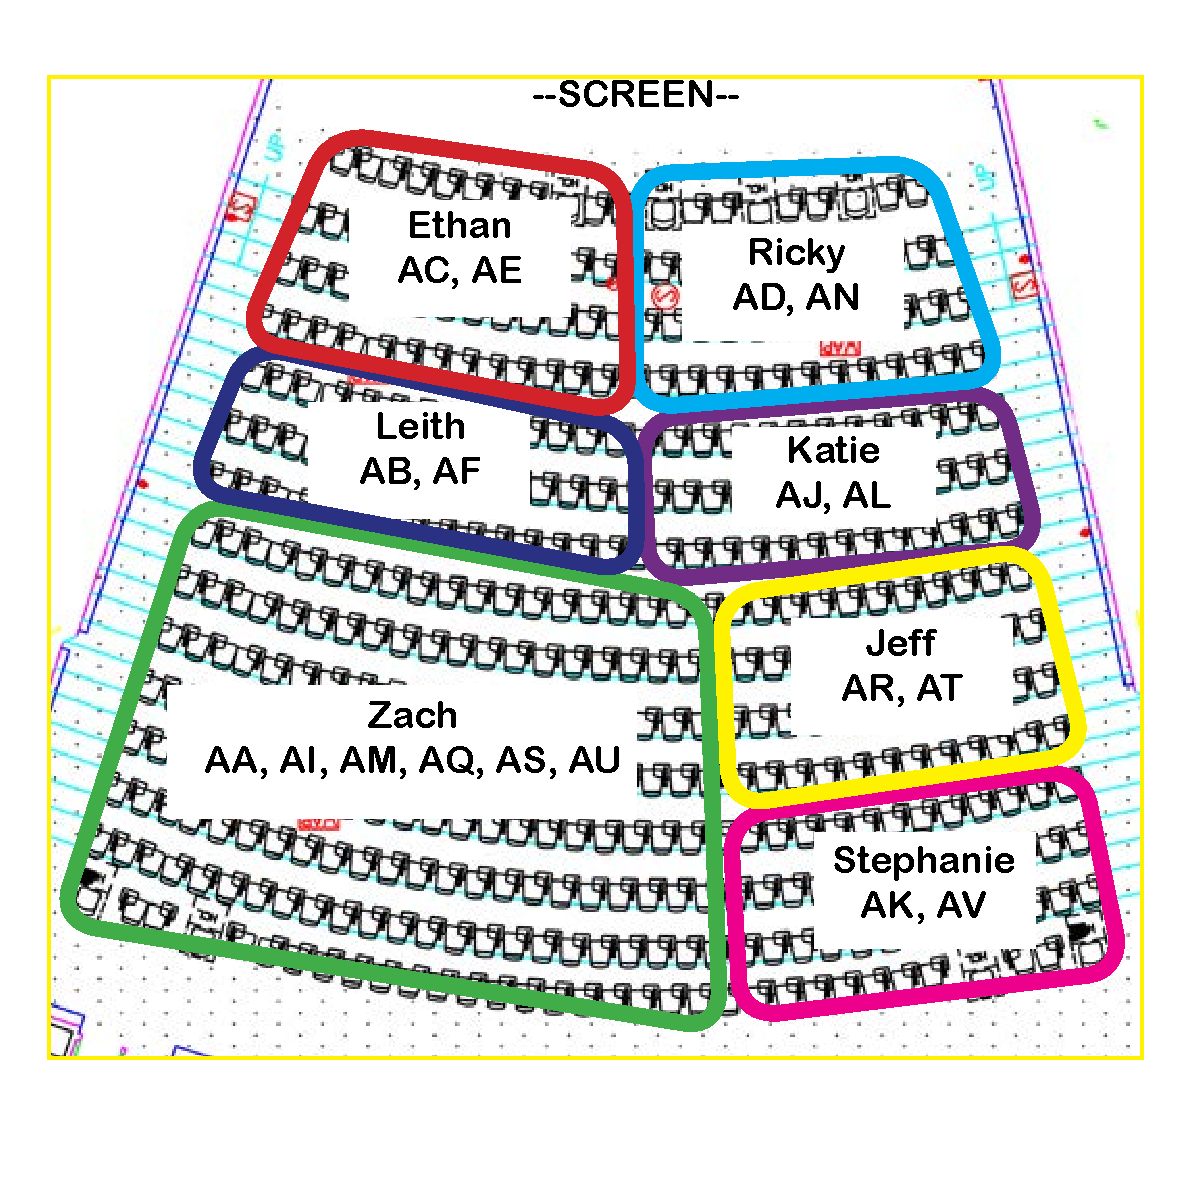
\includegraphics[height=1.3\textheight]{../images/seating-chart.pdf}
    \end{center}
\end{frame}
\end{noheadline}
}

\begin{noheadline}
\begin{frame}
    \begin{adjustwidth}{-2em}{-2em}
        \vspace{-5mm}
\includegraphics<1| handout:0>[page=1,width=\paperwidth]{./johns-slides.pdf}
\includegraphics<2| handout:0>[page=2,width=\paperwidth]{./johns-slides.pdf}
\includegraphics<3| handout:0>[page=3,width=\paperwidth]{./johns-slides.pdf}
\includegraphics<4| handout:0>[page=4,width=\paperwidth]{./johns-slides.pdf}
\includegraphics<5| handout:1>[page=5,width=\paperwidth]{./johns-slides.pdf}
\includegraphics<6| handout:0>[page=6,width=\paperwidth]{./johns-slides.pdf}
\includegraphics<7| handout:0>[page=7,width=\paperwidth]{./johns-slides.pdf}
\includegraphics<8| handout:0>[page=8,width=\paperwidth]{./johns-slides.pdf}
\includegraphics<9| handout:0>[page=9,width=\paperwidth]{./johns-slides.pdf}
\includegraphics<10| handout:2>[page=10,width=\paperwidth]{./johns-slides.pdf}
\includegraphics<11| handout:0>[page=11,width=\paperwidth]{./johns-slides.pdf}
\includegraphics<12| handout:3>[page=12,width=\paperwidth]{./johns-slides.pdf}
\includegraphics<13| handout:4>[page=13,width=\paperwidth]{./johns-slides.pdf}
\includegraphics<14| handout:0>[page=14,width=\paperwidth]{./johns-slides.pdf}
\includegraphics<15| handout:5>[page=15,width=\paperwidth]{./johns-slides.pdf}
    \end{adjustwidth}
\end{frame}
\end{noheadline}

% \begin{noheadline}
% \begin{frame}
%     \#ObserveEverything

%     \bigskip

%     \url{http://www.sciencefriday.com/teacher-resources/09/26/2014/science-club-observeeverything.html?interest=2&audience=4&series=34}
% \end{frame}
% \end{noheadline}

\blankslide

\begin{noheadline}
\begin{frame}
    \begin{clickerquestion}
        \item Suppose you wanted to do an experiment on how a new
            blood pressure medication affects the risk of stroke. How
            could you ensure that there was only one difference between
            the treatment groups, but still have the most meaningful data
            possible? 
        \begin{clickeroptions}
            \item \clickeranswer{Have the volunteers live normally, but use a
                    large sample and randomly assign the treatments.}
            \item Have the volunteers live in a hotel, where
                environmental variables can be carefully controlled. 
            \item Have the volunteers live normally, but record all
                environmental variables for each individual so you can
                factor them out. 
            \item Compare the treatments in identical twins (people
                who are genetically identical). 
        \end{clickeroptions}
    \end{clickerquestion}
\end{frame}
\end{noheadline}

\begin{noheadline}
\begin{frame}
\frametitle{Today's issues:}
\tableofcontents
\end{frame}
\end{noheadline}


\section{Non-experimental evidence in science}

\begin{frame}
    \begin{itemize}
        \item<1-> In lab next week, you will be considering the nature of
            experimental evidence.
        \item<2-> What other sorts of evidence do scientists use? 
        \begin{itemize}
            \item Astronomers:
                \wbox{radio waves, light emissions, imaging, modeling based on
                    known processes and forces}
            \item Geologists:
                \wbox{inference about past events from current
                    landforms/processes (e.g., glacial striations)}
        \end{itemize}
    \end{itemize}
\end{frame}
% Do the “shoes and belt exercise” here


\begin{frame}
    \begin{quote}
        \small
        All science textbooks purchased with state moneys must have the
        following notice placed prominently in them.

        This textbook discusses evolution, a controversial theory some
        scientists present as a scientific explanation for the origin of living
        things, such as plants, animals, and humans. 

        \highlight{No one was present} when life first appeared on earth.
        Therefore, any statement about life’s origins should be considered
        \highlight{as theory, not fact}.

        The word ``evolution'' may refer to many types of change. Evolution
        describes changes that occur within a species. (White moths, for
        example, may ``evolve'' into gray moths.) This process is
        microevolution, which can be observed and described as fact. 

        Evolution may also refer to the change of one living thing into
        another, such as reptiles into birds. \highlight{This process}, called
        macroevolution, \highlight{has never been observed and should be
            considered a theory}.
    \end{quote}
    \vspace{-2mm}
    \wbox{\small Theory = A testable explanation for a broad suite of observations;
        supported by a lot of evidence; generates new hypotheses}
\end{frame}
\note[itemize]{
    \item Highlight these passages in your notes.
    \item Focus on diff of theory in everyday English v biology/science
    \item Are theory and facts opposites? NO! Theories explain facts (data)!
        Explanation more powerful than data.
    \item Tennessee 1926 was the Scopes trial = illegal to teach evolution
    \item Louisiana 1987 was equal time legislation struck down by the US
        Supreme Court; Edwards v Aguillard
    \item Washington State Legislature introduced Senate Bill 6058 in 2002
    \item Washington State Senate Bill 6500 was even worse.
    \item Pennsylvania 2005  Dover trial
    \item Germ theory of disease, cell theory, theory of gravitation, atomic
        theory, heliocentric theory of the solar system
}
% First amendment


\begin{frame}
    \begin{itemize}
        \item Pasteur published the germ theory of disease in the 1860s; no one
            saw a virus until the 1950s.
        \item The atomic theory of matter was proposed in the early 1900s; no
            one saw an atom until the early 2000s.
        \item No one has seen a graviton, but you are not floating off into
            space!
    \end{itemize}

    How do these observations relate to the statements highlighted in purple on
    the previous slide?
    \begin{uncoverenv}<2->
    \begin{itemize}
        \item \href{http://www.pooprints.com/}{PooPrints} \ldots no joke!
            \note[item]<1>{Dog poo CSI}
    \end{itemize}
    \end{uncoverenv}
    \wbox{\small There was persuasive evidence to support these theories, even
        though the evidence was not ``eye-witness''}

    \vspace{1mm}
    \uncover<3->{What is a theory?}
    \wbox{\small An explanation for a broad class of phenomena that is
        supported by a lot of evidence}

\note[item]<2>{human perception as a model; our brain processes data to create a (very)
    subjective model of the world}
% Ask: Did OJ Simpson kill his estranged wife?
\end{frame}

\begin{frame}
    \begin{itemize}
        \item<1-> Science starts with a question
        \begin{itemize}
            \item ``The mystery of mysteries'': Where do species come from, and
                how have they come to be so well adapted to their environments?
                \note[item]<1>{Quote from John Herschel letter to Charles Lyell
                    about Lyell's Geology book}
        \end{itemize}
        \item<2-> Scientific theories usually have a pattern component and a
            process component
        \begin{itemize}
            \item The pattern component is
                \wbox{What we observe---``facts'' about the natural world---the
                    way things are: WHAT?}
                \vspace{1cm}
            \item The process component is
                \wbox{The process responsible for that pattern (underlying
                    mechanism, physical force or event):  HOW/WHY?}
        \end{itemize}
\end{itemize}
\end{frame}

\section{Plato/Aristotle/Special creation}

\begin{frame}
\frametitle{Today's issues:}
\tableofcontents[currentsection]
\end{frame}

\begin{frame}

    Process: \\

        \wbox{A supernatural being instantaneously and independently created all of
        the species observed today}
    \note[item]{Special creation aka scientific creationism aka intelligent design}
    
    \uncover<2->{Can the process component be tested? Why or why not?}
        \vspace{1mm}
        \wbox{No---it was a one-time supernatural occurrence}
        \vspace{1mm}
    
    \uncover<2->{Why is it called ``special'' creation?}
        \vspace{1mm}
        \wbox{It is not a natural process; it is supernatural}
        \vspace{1mm}
    

    \uncover<2->{Is it a valid scientific hypothesis or theory?}
        \vspace{1mm}
        \wbox{No---it lacks a testable natural process component}

\end{frame}

\begin{frame}

    Pattern:

    \begin{uncoverenv}<2->
    \begin{itemize}
        \item Special creation predicts:
        \begin{enumerate}[a)]
            \item Species are young
            \item Species are unrelated (created independently)
            \item Species are static
        \end{enumerate}
    \end{itemize}
    \end{uncoverenv}

\end{frame}

\begin{frame}

    Testing the prediction that (a) species are young:

    \begin{description}
        \item[Uniformitarianism] Processes occurring today also occurred in the
            past (e.g., sedimentation, erosion) 
            \wbox{Relative age---erosion and sedimentation are slow---long times
                required to create sandstones, chalk, mudstones, canyons, etc.}
            \note[item]{Hutton in late 1700s; Lyell in 1830}
        \item[Radiometric dating]
            \wbox{Absolute dating of rocks---age of the earth is
                $\approx$4.6 billion years; first life forms at $\approx$3.4 billion}
            \note[item]{Henri Becquerel; Marie Curie 1900s-current data}
    \end{description}

    What do uniformitarianism and radiometric dating have to say about the age
    of the Earth? \\



\end{frame}

\begin{frame}[t]

    Testing the prediction that (b) species are independent/unrelated:

    \begin{enumerate}
        \item Geographic relationships; e.g., Wallace's Line in Southeast Asia
        % Draw this
    \end{enumerate}

    \vspace{-2mm}
    \begin{center}
    \includegraphics<1| handout:1>[width=0.8\textwidth]{../images/se-asia-present.png}
    \includegraphics<2| handout:0>[width=0.8\textwidth]{../images/se-asia-120.png}
    \end{center}
\end{frame}
\note[itemize]{
\item Many other island groups with similar patterns
\item Anolis lizards in Caribbean
\item Fruit flies and silverswords in Hawaii
}


\begin{frame}
    \begin{clickerquestion}
        \item What does special creation predict about the
            geographic relationships of closely related species? 
        \begin{clickeroptions}
            \item Similar species should be found in the same geographic area.
            \item Species that look similar should be found in similar
                habitats, no matter where they are in terms of geography.
            \item In terms of geography, species that look similar should be
                distributed at random. 
            \item \clickeranswer{No specific predictions (species are found
                    where they are because God wanted them that way).}
        \end{clickeroptions}
    \end{clickerquestion}

    \wbox{What predictions does the theory of special creation make?  Problem:
        can't test the predictions (this is unscientific)}
\end{frame}

\begin{frame}[t]

    Testing the prediction that (b) species are independent/unrelated:

    \begin{enumerate}[\begingroup 2.\endgroup]
        \item Homology (``same source'') = similarities in form among species
            (e.g., timber wolf, Ethiopian wolf, \ldots dog)
    \end{enumerate}

    \vspace{-3mm}
    \begin{uncoverenv}<2->
    \begin{center}
    \includegraphics[height=2.9cm]{../images/canis-lupus.jpg}\hspace{0.1mm}
    \includegraphics[height=2.9cm]{../images/canis-simensis.jpg}\hspace{0.1mm}
    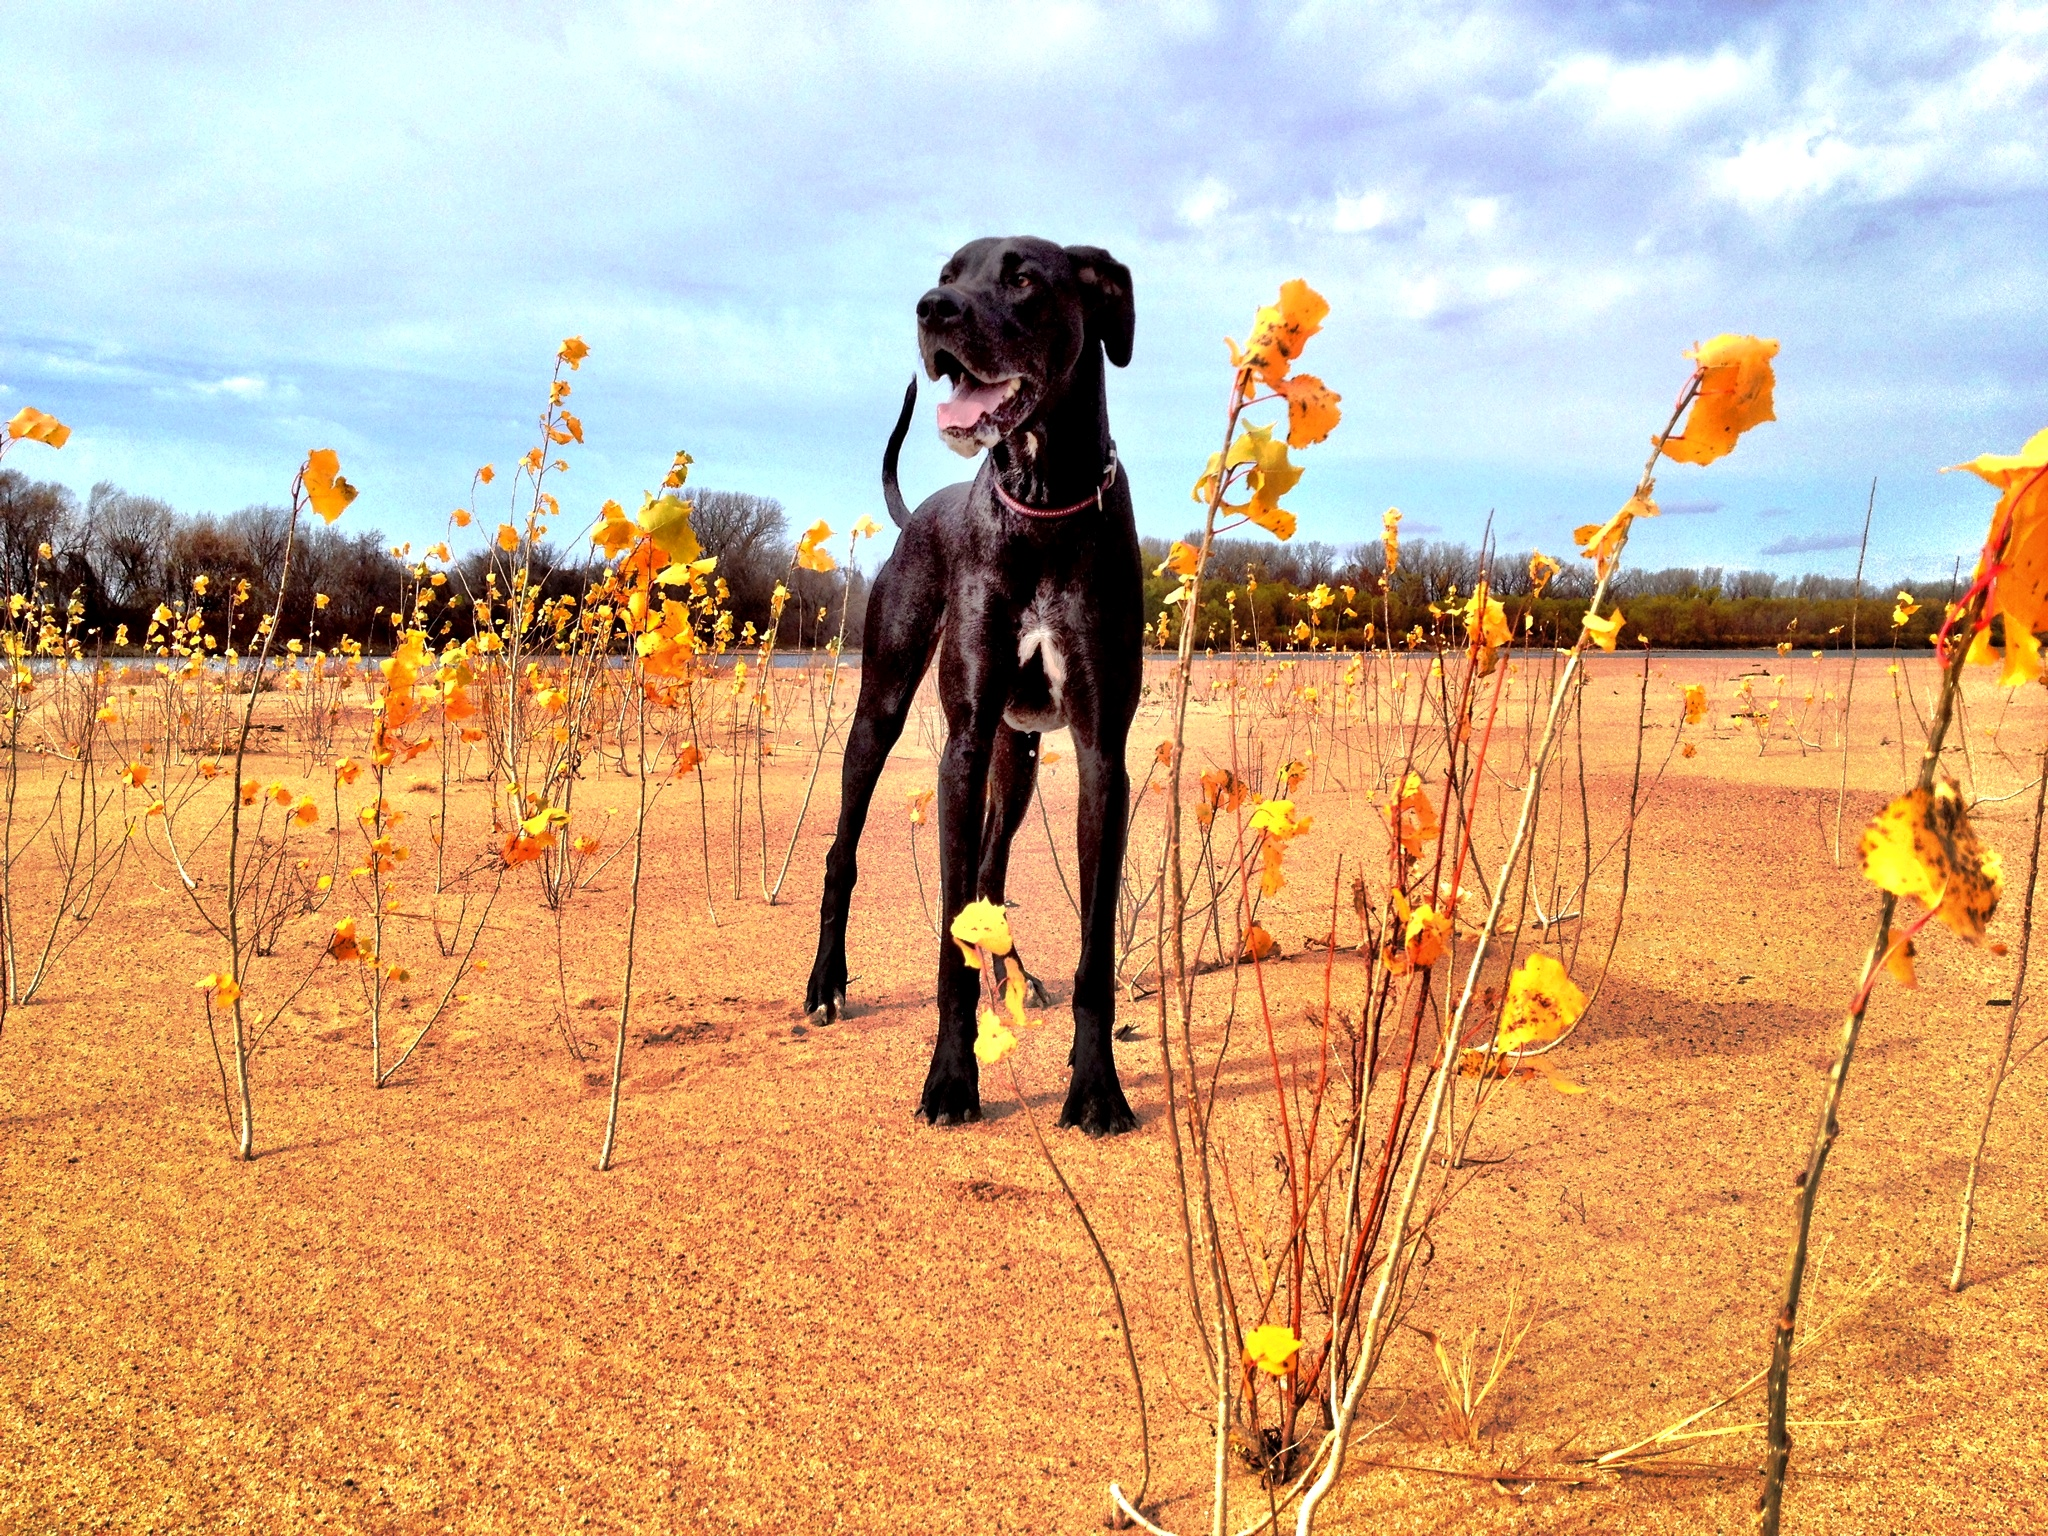
\includegraphics[height=2.9cm]{../images/luna.jpg}
    % \includegraphics[height=2.7cm]{../images/thylacinus.jpg}
    \end{center}
    \end{uncoverenv}

    \vspace{-3mm}
    \uncover<3->{
    Why are timber wolves, Ethiopian wolves, and dogs extremely similar at the
    genetic, developmental, and structural levels?
    \wbox{Divine intervention? Or, because they are closely related; they
        inherited traits from an ancestor}
    }
    \note[item]{Africa's most endangered carnivore}
\end{frame}

\begin{frame}

    Testing the prediction that (c) species are static:

    \begin{enumerate}
        \item Extinction/the law of succession:
            \vspace{1cm}
        \item Transitional features:
            \vspace{1cm}
        \item Vestigial traits:
            \vspace{1cm}
        \item Evolution in action:
    \end{enumerate}

    \wbox{Find examples of each pattern above. Are these patterns more
        consistant (predicted by) special creation or evolution by natural
        selection? What do they say about the internal consistency of
        evolution?}

    % Succession is like geographic relationships, except add element of time

    % In general: under evolution by natural selection, all of these patterns
    % are logical---under special creation, they are puzzling

    % Scientific theories are considered powerful if they explain otherwise
    % puzzling observations

    % Internal consistency!! Predictions supported by many independent sourced
    % of data
\end{frame}

\begin{frame}
    \begin{clickerquestion}
        \item Plant cells have 3 types of genomes (nucleus, mitochondria, and
            chloroplast) that are inherited independently. From each, we can
            estimate the relationships among
            species based on similarities and differences in homologous DNA
            sequences. If species evolve (share ancestry), what pattern
            is predicted?
        \begin{clickeroptions}
            \item The relationships will be the same for the mitochondria and
                chloroplast, but different for the nuclear genome. 

            \item The relationships among plant species will be different for
                each genome.

            \item \clickeranswer{The relationships among plant species will be
                    the same for all 3 genomes.}

            \item No specific pattern is predicted. 
        \end{clickeroptions}
    \end{clickerquestion}
    % What predictions does the theory of special creation make?
    % Problem: can't test the predictions (this is unscientific)
\end{frame}

\begin{frame}
    Current consensus among working scientists and mainstream theologians:

    \begin{itemize}
        \item<2-> Science deals with questions that can be answered by going out
            and measuring something.
        \item<3-> Religion deals with questions that cannot be answered by
            measuring something. 
        \item<4-> By definition\footnote{\scriptsize Webster’s Encyclopedic Unabridged
                Dictionary of the English Language, 1966}, belief and faith
            (including religious belief and faith) do not depend on evidence. 
    \end{itemize}
\end{frame}
\note[itemize]{
    \item This is the distinction between science, pseudoscience, and
        religion
    \item There is no conflict between science and religion---except for
        literal interpretation of the creation story of the Book of Genesis
    \item US courts have always said No
}

\section{``Lamarckian'' evolution}

\begin{frame}
\frametitle{Today's issues:}
\tableofcontents[currentsection]
\end{frame}

\begin{frame}
    Pattern:
    \begin{itemize}
        \item Key claim is that evolutionary change is
            \wbox{progressive---leads to ladder of life}
    \end{itemize}

    \bigskip
    Process:
    \begin{itemize}
        \item Key claim is that \highlight{individuals} change in
            response to changes in the environment, and
            \wbox{pass those changes on to offspring. As a result the
                characteristics of populations change through time}
    \end{itemize}
\end{frame}

\begin{frame}
    \begin{clickerquestion}
        \item Under the theory of evolution as formulated by Lamarck, why would
            the traits of Pacific oysters change in response to ocean
            acidification?
        \begin{clickeroptions}
            \item \clickeranswer{Individuals in low pH conditions would grow
                    shells more efficiently in response. These changes would be
                    passed on to offspring.}

            \item Individuals that happened to be more efficient at
                shell-building would have more offspring than others, so the
                characteristics of the population would change over time.

            \item A supernatural power would make the oysters more efficient at
                shell-building in acidic conditions, so they would adapt. 
 
            \item Oysters would be eliminated from low pH habitats, and only be
                found in higher pH habitats. 
        \end{clickeroptions}
    \end{clickerquestion}
\end{frame}

\end{document}

